\chapter{Практический раздел}

\section{Базовые структуры вершины и правила}

\begin{lstlisting}
struct Node {
    int number;
    bool forbidden = false;
    bool closed = false;
};

struct Rule {
    std::vector<int> srcNodes;
    int dstNode;
    int number;
    bool visited = false;
    bool forbidden = false;
    unsigned int openIndex = 0;
};
\end{lstlisting}

\section{Класс поиска в графе}

\begin{lstlisting}
class GraphSearch {
public:
    GraphSearch(std::list<Rule> rules, std::vector<int> srcNode, int dstNode);
    std::list<int> DoDepthFirstSearch();

private:
    int DescendantsDFS(int node);
    void Backtrack(int node);
    void Mark(int node);

    std::list<Rule> m_rules;
    std::map<int, Node> m_nodes;
    std::map<int, Rule *> m_rulesRef;
    std::list<int> m_openNodes;
    std::list<int> m_openRules;
    std::list<int> m_closedNodes;
    std::list<int> m_closedRules;
    std::vector<int> m_srcNodes;
    bool m_foundSolution = false;
    bool m_noSolution = false;
};
\end{lstlisting}

\section{Реализация методов класса поиска}

\begin{lstlisting}
GraphSearch::GraphSearch(std::list<Rule> rules, std::vector<int> srcNodes, int dstNode) : m_rules(std::move(rules)), m_srcNodes(std::move(srcNodes)) {
  if (m_srcNodes.size() == 0)
    m_noSolution = true;
  else if (std::find(m_srcNodes.begin(), m_srcNodes.end(), dstNode) != m_srcNodes.end())
    m_foundSolution = true;
  else {
    for (auto node : m_srcNodes) {
      m_nodes[node].closed = true;
      m_closedNodes.push_back(node);
    }
    for (auto &rule : m_rules)
      m_rulesRef[rule.number] = &rule;
    m_openNodes.push_back(dstNode);
  }
}

std::list<int> GraphSearch::DoDepthFirstSearch() {
  while (!m_foundSolution && !m_noSolution) {
    int node = m_openNodes.back();
    int count = DescendantsDFS(node);
    if (m_foundSolution) {
      Mark(node);
      if (m_foundSolution) break;
    } else if (count == 0 && !m_openNodes.empty()) {
      Backtrack(node);
    } else if (m_openNodes.empty()) {
      m_noSolution = true;
      break;
    }
  }
  return m_noSolution ? {} : m_closedRules;
}

int GraphSearch::DescendantsDFS(int node) {
  int count = 0;
  for (auto &rule : m_rules) {
    if (rule.visited || rule.dstNode != node || rule.forbidden)
      continue;
    bool all_closed = true;
    for (auto srcNode : rule.srcNodes) {
      const Node &nodeRef = m_nodes[srcNode];
      if (nodeRef.forbidden) {
        rule.forbidden = true;
        break;
      }
      all_closed = all_closed && nodeRef.closed;
    }
    if (rule.forbidden) continue;
    m_openRules.push_back(rule.number);
    if (all_closed) {
      m_foundSolution = true;
      break;
    }
    m_rulesRef[rule.number]->openIndex = m_openNodes.size();
    for (auto srcNode : rule.srcNodes)
      if (!m_nodes[srcNode].closed)
        m_openNodes.push_back(srcNode);
    rule.visited = true;
    ++count;
  }
  return count;
}

void GraphSearch::Backtrack(int node) {
  while (true) {
    // node at top of open node stack needs to be forbidden
    m_nodes[node].forbidden = true;
    // then rule at top of open rules stack needs to be forbidden
    if (m_openRules.empty()) {
      m_noSolution = true;
      break;
    }
    int ruleNum = m_openRules.back();
    Rule *ruleRef = m_rulesRef[ruleNum];
    int dstNode = ruleRef->dstNode;
    ruleRef->forbidden = true;
    //  all input nodes of that rule must be removed from open nodes
    for (const auto &rule : m_rules) {
      if (rule.number == ruleNum) {
        while (ruleRef->openIndex < m_openNodes.size())
          m_openNodes.pop_back();
        break;
      }
    }
    m_openRules.pop_back();
    // new open rule must be searched to close previous node in open stack
    // 1. check if previous open rule resolves current top of open nodes
    // 2. if true - continue with this rule
    //    if not - remove this rule and corresponding nodes and retry
    if (m_openRules.empty())
      m_noSolution = true;
    else if (m_rulesRef[m_openRules.back()]->dstNode == dstNode)
      break;
    node = dstNode;
  }
}

void GraphSearch::Mark(int node) {
  // 0. mark given node as closed
  // 1. pop all rules that have same dst node
  // 2. if current top of opened rules has closed inputs - repeat
  // 3. dont forget to update m_foundSolution variable if real solution was found!
  while (m_foundSolution) {
    m_nodes[node].closed = true;
    m_closedNodes.push_back(node);
    m_closedRules.push_back(m_openRules.back());
    while (!m_openRules.empty() && m_rulesRef[m_openRules.back()]->dstNode == node)
      m_openRules.pop_back();
    // real solution found
    if (m_openRules.empty())
      return;
    // remove all open nodes up until given node
    while (m_openNodes.back() != node)
      m_openNodes.pop_back();
    m_openNodes.pop_back();
    // check current top
    int rule = m_openRules.back();
    bool all_closed = true;
    for (auto srcNode : m_rulesRef[rule]->srcNodes) {
      if (!m_nodes[srcNode].closed) {
        all_closed = false;
        break;
      }
    }
    if (all_closed)
      node = m_rulesRef[rule]->dstNode;
    else m_foundSolution = false;
  }
}
\end{lstlisting}

\clearpage

\section{Тестирование ПО}

Для тестирования реализации алгоритма поиска была составлена база знаний, соответствующая графу, представленному на рисунке \ref{fig:graph0}.

\begin{figure}[h!]
    \centering
    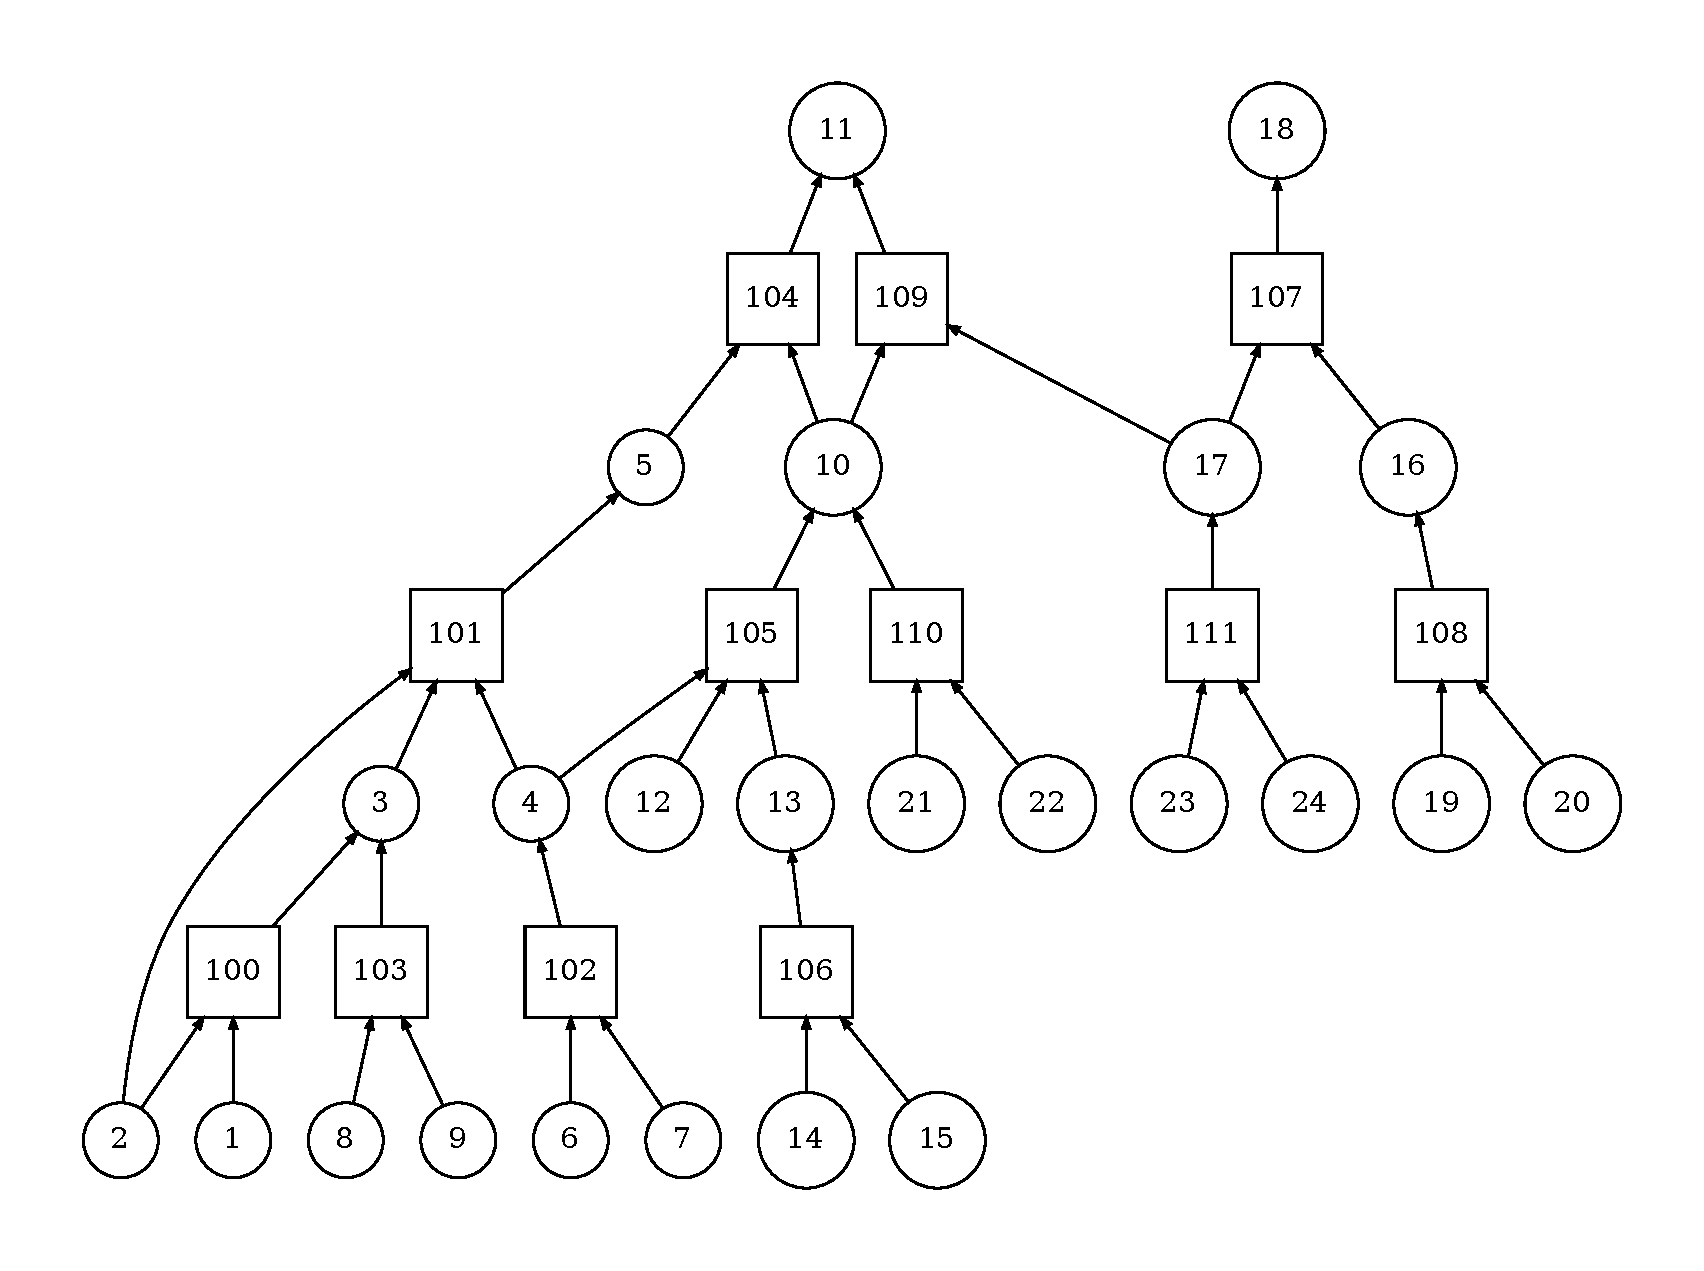
\includegraphics[width=\linewidth]{img/kb.pdf}
    \caption{Граф составленной базы знаний}
    \label{fig:graph0}
\end{figure}

\begin{table}[h!]
    \centering
    \caption{Тестовые данные для проверки реализации алгоритма}
    \begin{tabular}{|c|c|c|c|}
        \hline
        Входные & Выходная & Ожидаемый & Фактический \\
        вершины & вершина & результат & результат \\
        \hline
        \hline
        $1,2,4,8,9$ & $5$ & $100,101$ & $100,101$ \\
		$2,3,4,12,13,21,22,23,24$ & $11$ & $111,105,109$ & $111,105,109$ \\
		$8,9,6,7,12$ & $10$ & $\O$ & $\O$ \\
		$2,3,4,12,14,15,23,24$ & $11$ & $111,106,105,109$ & $111,106,105,109$ \\
        \hline
    \end{tabular}
\end{table}
